%!TEX root = ../../secondYearReport.tex
 
\paragraph{Work package 3 progress}

The progress for each task is described hereafter.

\subparagraph{Formulating the control problem (T3.2) (UPMC: 3PM)}

During Year 2, UPMC has explored the different possible usage of the Generalized Hierarchical Controller developed in Year 1 \cite{LiuGHC} and allowing the specification of both strict and soft hierarchical control problems. In \cite{LiuAutRobSpecIssue}, a quasi-static version of this controller is used in simulation for a standing scenario where the iCub robot is using an additional contact which is switched from one hand to the other. This control architecture has also been successfully applied on a KUKA LWR robot \cite{LiuICRA2015}. Tasks performances for three conflicting tasks are illustrated on Figure~\ref{fig:KUKA_LWR_GHC}.

\begin{figure*}[h!]
\centering
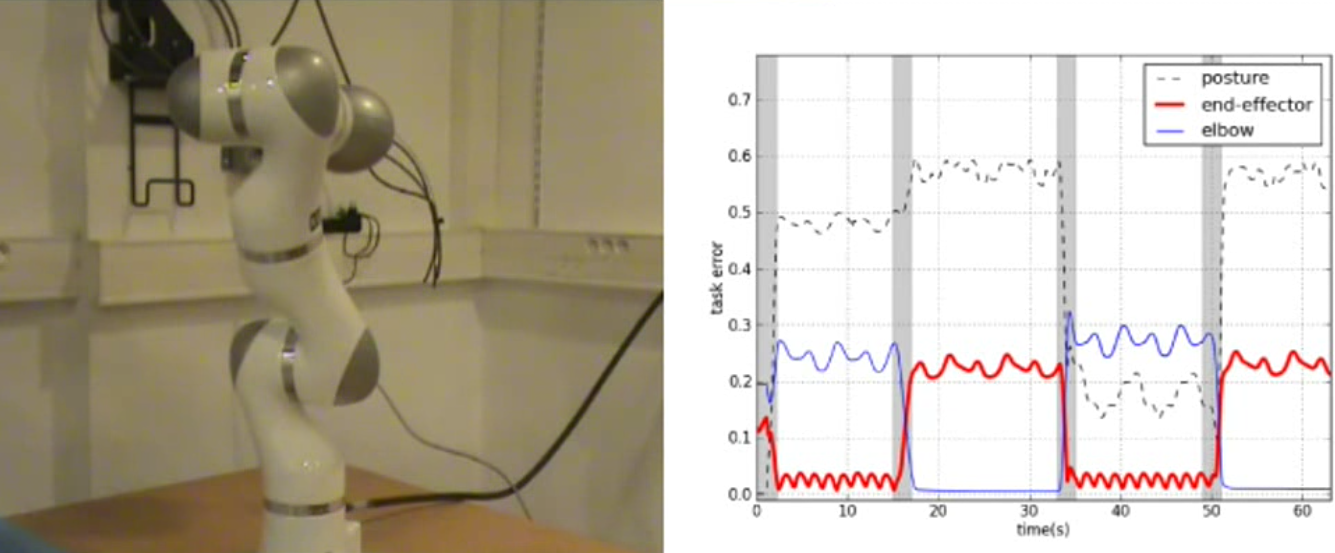
\includegraphics[width=0.65\textwidth]{images/KUKA_GHC_ICRA}
\caption{Tasks performance for three conflicting tasks using the GHC control framework.}
\label{fig:KUKA_LWR_GHC}
\end{figure*}

\subparagraph{Solving the local control problem (T3.3) (UPMC: 4.5PM, UB: 0.9PM, TUD: 2.5PM)}

During Year 2, UPMC has started to investigate scenarios where the robot is interacting with the environment through rigid and non-rigid contacts. Assuming that no information is a priori available regarding the nature of the contact surface, a first control strategy has been proposed in \cite{LiuIROS2015} where the desired contact force is adapted online as a function of the velocity of the contact point. Indeed, the risk with an unknown contact surface is to assume that it will almost instantaneously provide the required contact force to maintain the robot balance. If the surface is non-rigid, the contact point will actually move while being pushed and stable support forces will only be provided to the robot once the contact is properly established. The goal of the adaptation of the desired value for the contact force is to accelerate the obtainment of a stable contact force supporting the robot. The desired trajectory for the center of mass of the robot is also adapted to account for the non-rigidity of the contact surface. One of the advantages of this approach is that it does not actually requires the knowledge of the contact surface impedance. Figure~\ref{fig:LIU_IROS_2015} provides a view of the types of considered scenarii and the structure of the considered controller. In this work, the local control problem is solved using the solver described in \cite{salini2012} rather than the one developed in \cite{LiuGHC}. This choice is related to the fact that the computation cost of the GHC approach remains important and is too high to be actually used in a real-time reactive control architecture for a humanoid robot.\\

\begin{figure*}[h!]
\centering
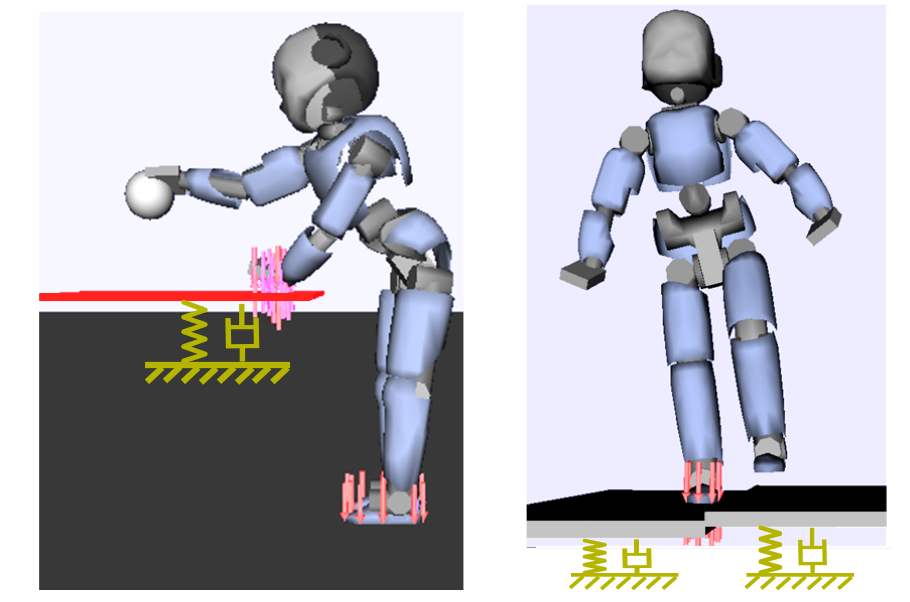
\includegraphics[width=0.45\textwidth]{images/LIU_IROS_2015} 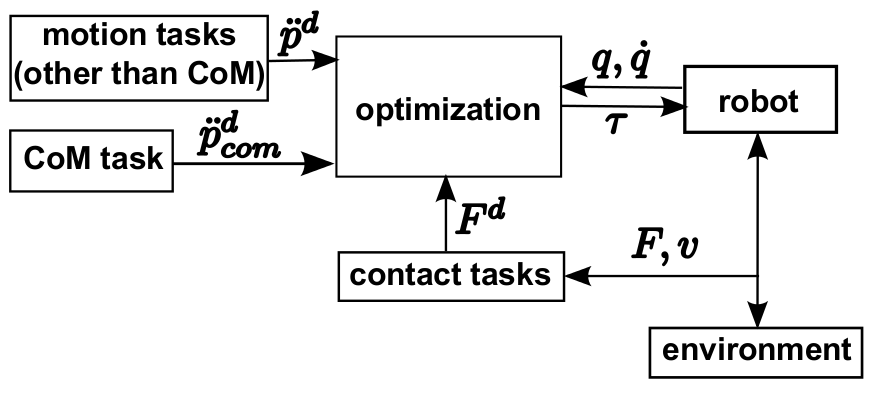
\includegraphics[width=0.45\textwidth]{images/LIU_IROS_2015_bis}
\caption{Scenarri of interaction with a non-rigid environment (\textit{left}). Structure of the adaptive control architecture (\textit{right}).}
\label{fig:LIU_IROS_2015}
\end{figure*}

In the meantime, UB proposed an algorithm for implementing a momentum
based controller to control balancing motion of legged robots with non-rigid
contacts with the environments \cite{Azad&Mistry15}.  The proposed strategy
converts the balance problem to a linear constrained optimization problem
which its output is the vector of desired joint accelerations.  It first
calculates the desired supporting forces at the contact points by using the
robot’s momentum.  Then, based on the contact model and by using the Jacobian
of the contact points, it converts the desired contact forces to the desired
joint accelerations.  At the end, by using the inverse dynamics of the robot,
the joint torques are calculated.  To implement the proposed method in
practice, stiffness and damping coefficients of the contact model have to be
estimated beforehand by using contact model parameter estimation methods.\\
    
In order to best use the whole-body controllers developed within the framework of WP3, TUD hired a student for setting up the iCub hardware and simulation environment.


\subparagraph{Bootstrapping and validating the control approach in rigid world and compliant cases (T3.4) (IIT: 3PM, UPMC: 7.19PM, UB: 0.95PM, TUD: 8PM, JSI: 1PM, Inria: 4PM)}

During Year 2, the whole-body controller developed by UPMC and originally described in \cite{salini2012} has been ported, using the Whole Body Interface described in Deliverable~D1.2, on the iCub robot. A non-free-floating first implementation was performed during the \textit{Veni, Vidi, Vici} 2014 summer school. The free-floating version is less straightforward as it requires: a well calibrated torque low-level control loop and a proper on-line estimation of the state of the root-body in order to  compute the dynamics and kinematics models of the robot\footnote{The retained solution is to choose one body in contact with the fixed environment as the root-body (one foot for example) and switch the root-body whenever there is a switch in the contact state of the system.}. IIT is working on these two topics and UPMC, in coordination with IIT, is pursuing integration on its iCub robots.

UPMC also kept exploring the contribution of MPC approaches to  handle the postural balancing under varying contact conditions. The contributions in this domain are related to the thesis work of A. Ibanez \cite{ibanezIROS2014} and the postdoctoral work of D. Lau\footnote{A paper has been submitted to a conference with double blind reviews and cannot be explicitly referred to for obvious reasons.}.  In order to compute optimal time, duration and position of footsteps along with the center of mass trajectory of a humanoid, a novel mixed-integer model of the system is introduced in the work of A. Ibanez. The introduction of this model in a predictive control problem brings the definition of a Mixed-Integer Quadratic Program, subject to linear constraints. Simulation results demonstrate the simultaneous adaptation of the gait pattern and posture of the humanoid, in a walking activity under large disturbances, to efficiently compromise between task performance and balance. In addition, a push recovery scenario displays how, using a single balance-performance ratio, distinct behaviors of the humanoid can be specified. Results have been obtained in simulation\footnote{A video associated to this work can be found \href{http://pages.isir.upmc.fr/~padois/website/fichiers/videos/ibanez\_IROS2014.mp4}{here}.} and are being implemented on the TORO robot developed at DLR. This work is also being adapted in order to test control hypothesis to explain the behaviours observed in the experiment developed in T2.4 of WP2\footnote{This adaptation has been discussed during the visit of Jan Babic as an invited professor during November 2014 at  UPMC}. In the work of D. Lau, two simple and novel approaches to solve for 3D locomotion with multiple non-coplanar contacts are introduced. Both formulations use model predictive control to generate dynamically balanced trajectories with no restrictions on the center of mass height trajectory. The first formulation treats the balance criterion as an objective function, and solves the control problem using a sequence of alternating convex quadratic programs, while the second formulation considers the criterion as constraints to the problem, and solves a succession of convex quadratically constrained quadratic programs. Preliminary results have been obtained in a scenario where a hand contact on a vertical wall is used to improve balance. A staircase climbing scenario has also been studied.

In coordination with T4.4 in WP4, UPMC also explored ways to optimize tasks trajectories \cite{lober-HUMANOIDS2014} and the weights of tasks \cite{lobersubmittedIROS2015} in the LQP whole-body controller in order to maximize the overall control performance. More details are provided in the description of T4.4.\\

Continuing the activities which started in the first year of the project, IIT further improved the torque whole-body controller. During the second year of the project, attention was mainly on rigid contacts even if the theoretical and software development was guided and constrained by the requirements for extending the approach to non-rigid contacts. Several improvements to the controller significantly improved its performances. Improvements include in-situ force/torque sensor calibration \cite{Traversaro2015b}, inertial parameter identification \cite{Traversaro2015} and individual motor transfer function identification \cite{Nori2015a}. These improvements made possible quite challenging control tasks like the robust single foot balancing represented in Figure~\ref{fig:footBalancing}. Details of the controller will be given in a forthcoming publication.\\

\begin{figure}[h!]
\centering
{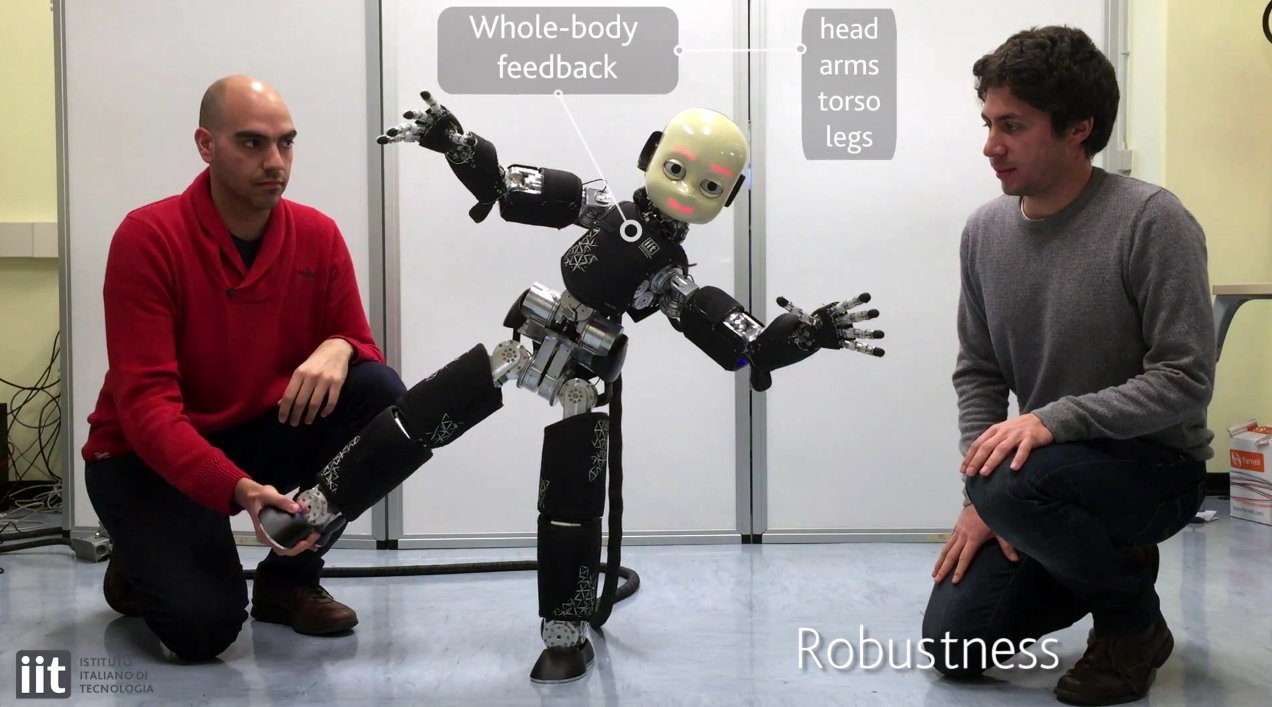
\includegraphics[width=0.65\textwidth]{images/single_foot_balancing.jpg}}
\caption{The picture shows the iCub while performing compliant single foot balancing. Details on the controller can be found in \cite{Nori2015a}. A video of the task is available on youtube\protect\footnotemark.}
\label{fig:footBalancing}
\end{figure}

\footnotetext{\url{https://www.youtube.com/watch?v=SYVCbzGsBF4}.}


During the second year, TUD continued their research in inverse dynamics model
learning in situations with contacts. A mixture of experts approach with
Gaussian processes was developed using tactile feedback from the iCub's sensor
skin. This approach was evaluated on the iCub robot, where the learned model
accurately predicts contact forces, is robust to changes in the environment and
outperforms existing analytic dynamic models that make use of force/torque
sensor data. 
An exemplary task is illustrated in Figure~\ref{fig:exp3:icuparis_experiment_bars} 
when obstacles are introduced on both sides of a planned circular motion.
In Figure~\ref{fig:exp3:gating} can be seen that the mixture-of-experts recognize the presence of the two different contacts and opportunely active the corresponding expert to compensate for the contact.
As a result, the torques predicted from this approach (red curve) closely follow the ground truth (blue curve) and outperform the analytic model (green curve).
A paper was published in an international robotics conference
\cite{Calandra_ICRA15}. A study exploiting learned dynamics models
for control is in progress of writing. Both studies are detailed in Deliverable
D4.2.\\

	\begin{figure}[t]
		\begin{minipage}{.43\linewidth}
			\centering
			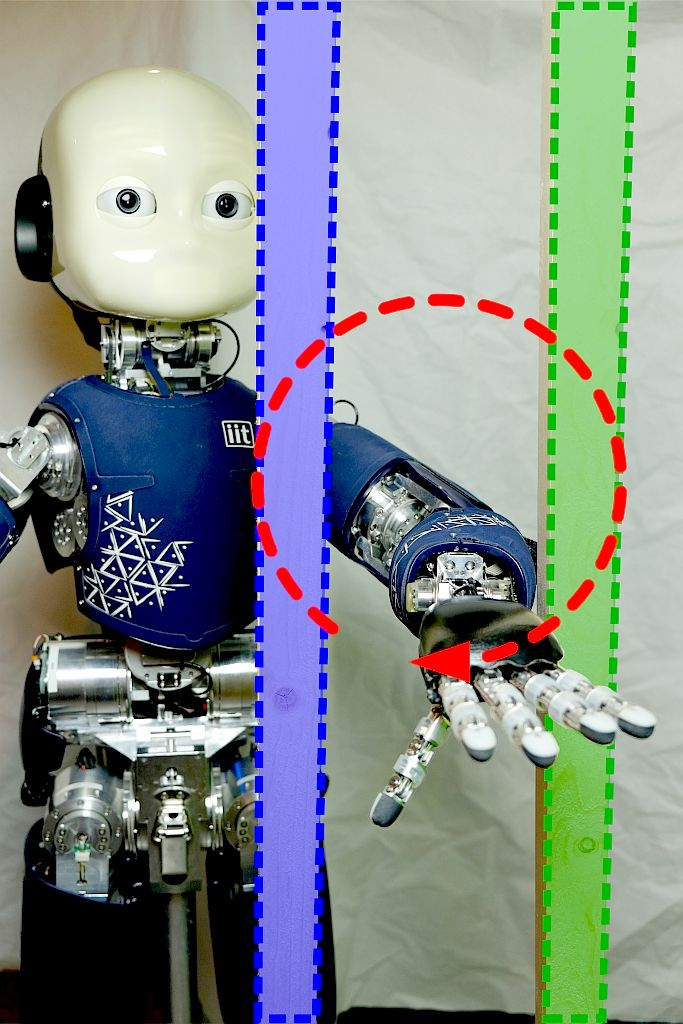
\includegraphics[width =.94\linewidth]{iCubParis02_Double_Contact}
			\caption{The robot performs a circle with its left arm. 
			The forearm collides alternatively with the left, the right or both contacts.}
			\label{fig:exp3:icuparis_experiment_bars}
		\end{minipage}	
		\hfill
		\begin{minipage}{.52\linewidth}
			\centering
			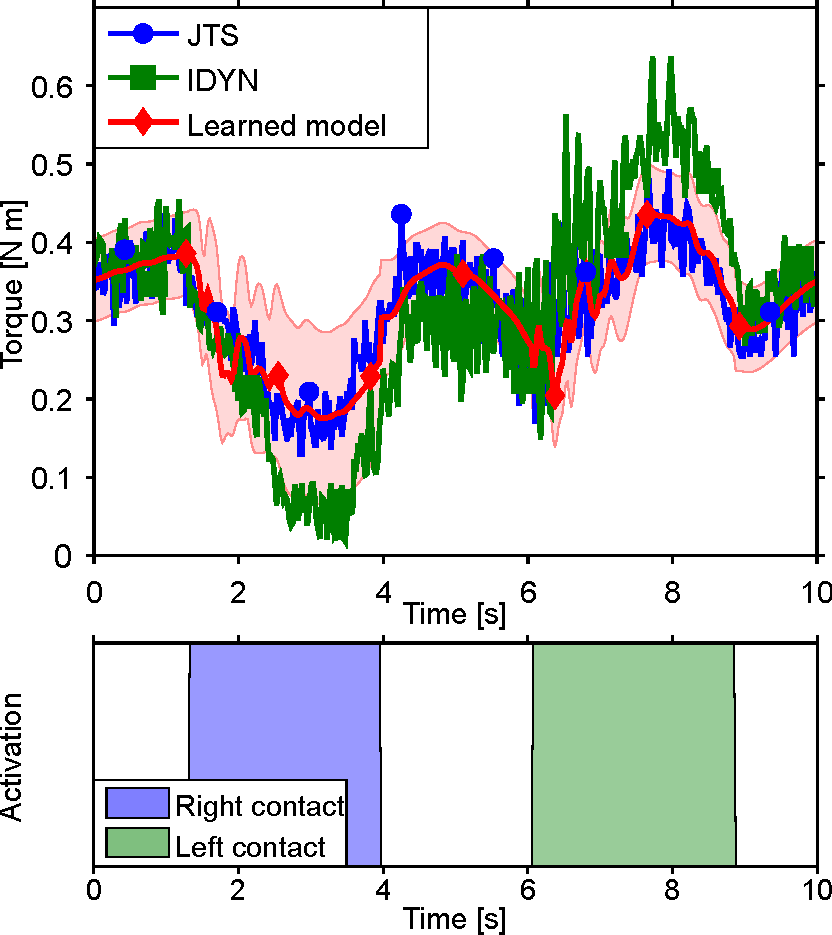
\includegraphics[width=.89\linewidth]{exp3_both}
			\caption{Prediction of torques with multiple contacts and the corresponding activation of the gating network.
			%Various models are shown, but individually, none of them correctly capture the dynamics of the system. 
			Our mixture-of-experts model combines the learned single-contact models into a multiple-contact model which outperform the analytic approach.
			}
			\label{fig:exp3:gating}
		\end{minipage}	
        %\figspace
	\end{figure}
	
INRIA, in collaboration with TUD, started to study the problem of bootstrapping the parameterized controllers proposed in T3.3. A major problem is how the controllers parameters, particularly the task weights, can be initialized or learned through trial-and-error. With the increasing abilities of humanoid robots, the number of tasks increases, together with their weights or priorities: manually specifying them through a sequence of complex manipulations becomes a major bottleneck. 
As a first step towards the offline optimization of those parameters, Inria evaluated the benefit of using a stochastic optimization derivative-free strategy such as \textit{Covariance Matrix Adaptation Evolution Strategy} (CMA-ES) \cite{Hansen-2001-ID362}. Figure~\ref{fig:robust} provides a view of the robustness of the optimization strategy by comparing several optimizations experiments with constant and random values for the GHC controller.
The full study is detailed in the Task 4.4.\\

\begin{figure}[h!]
  \centering
  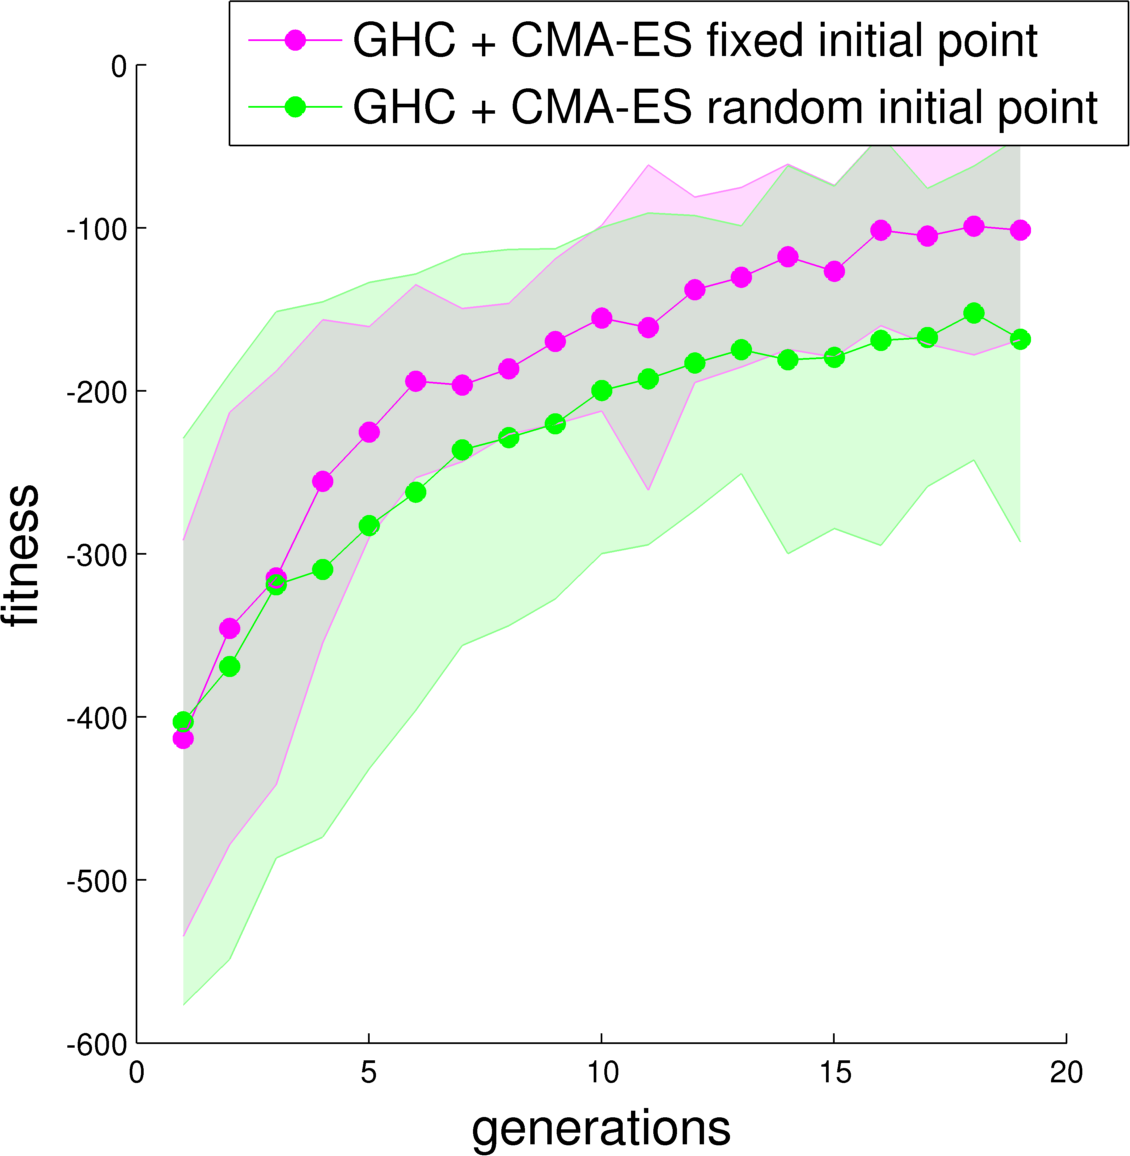
\includegraphics[width=0.5\hsize]{GHC_robust}
\caption{Learning the activation policies for GHC with CMA-ES. The policies were initialized with constant values $\alpha=0.5$ or random values between $[0,1]$. The mean and variance of the fitness function used for optimization for $R=20$ replicates a test experiment (see also Task 4.4).}
\label{fig:robust}
\end{figure}

In the meantime, UB also studied the problem of constrained motion for a manipulator performing
a task while in contact with the environment, and proposed a solution based on
projected operational space dynamics \cite{Ortenzietal14}.  The main
advantages of this control technique are: 1) it exploits the environment
contact constraint itself, so as to minimise the joint torques needed to
perform the task; 2) it enables full decoupling of motion and force control;
3) force feedback from a force sensor mounted at the end effector or other
contact points is not needed.  This work is a step towards a robot control
strategy which mimics the human behaviour of exploiting contacts with the
environment to help perform tasks.  They also presented an experimental
implementation of the control method in which a KUKA LWR IV manipulator used
an eraser to wipe a whiteboard.  They showed that the proposed controller can
effectively exploit contact with the whiteboard in order to reduce joint
torques while still performing the desired wiping motion.

\begin{figure*}[h!]
  \centering
  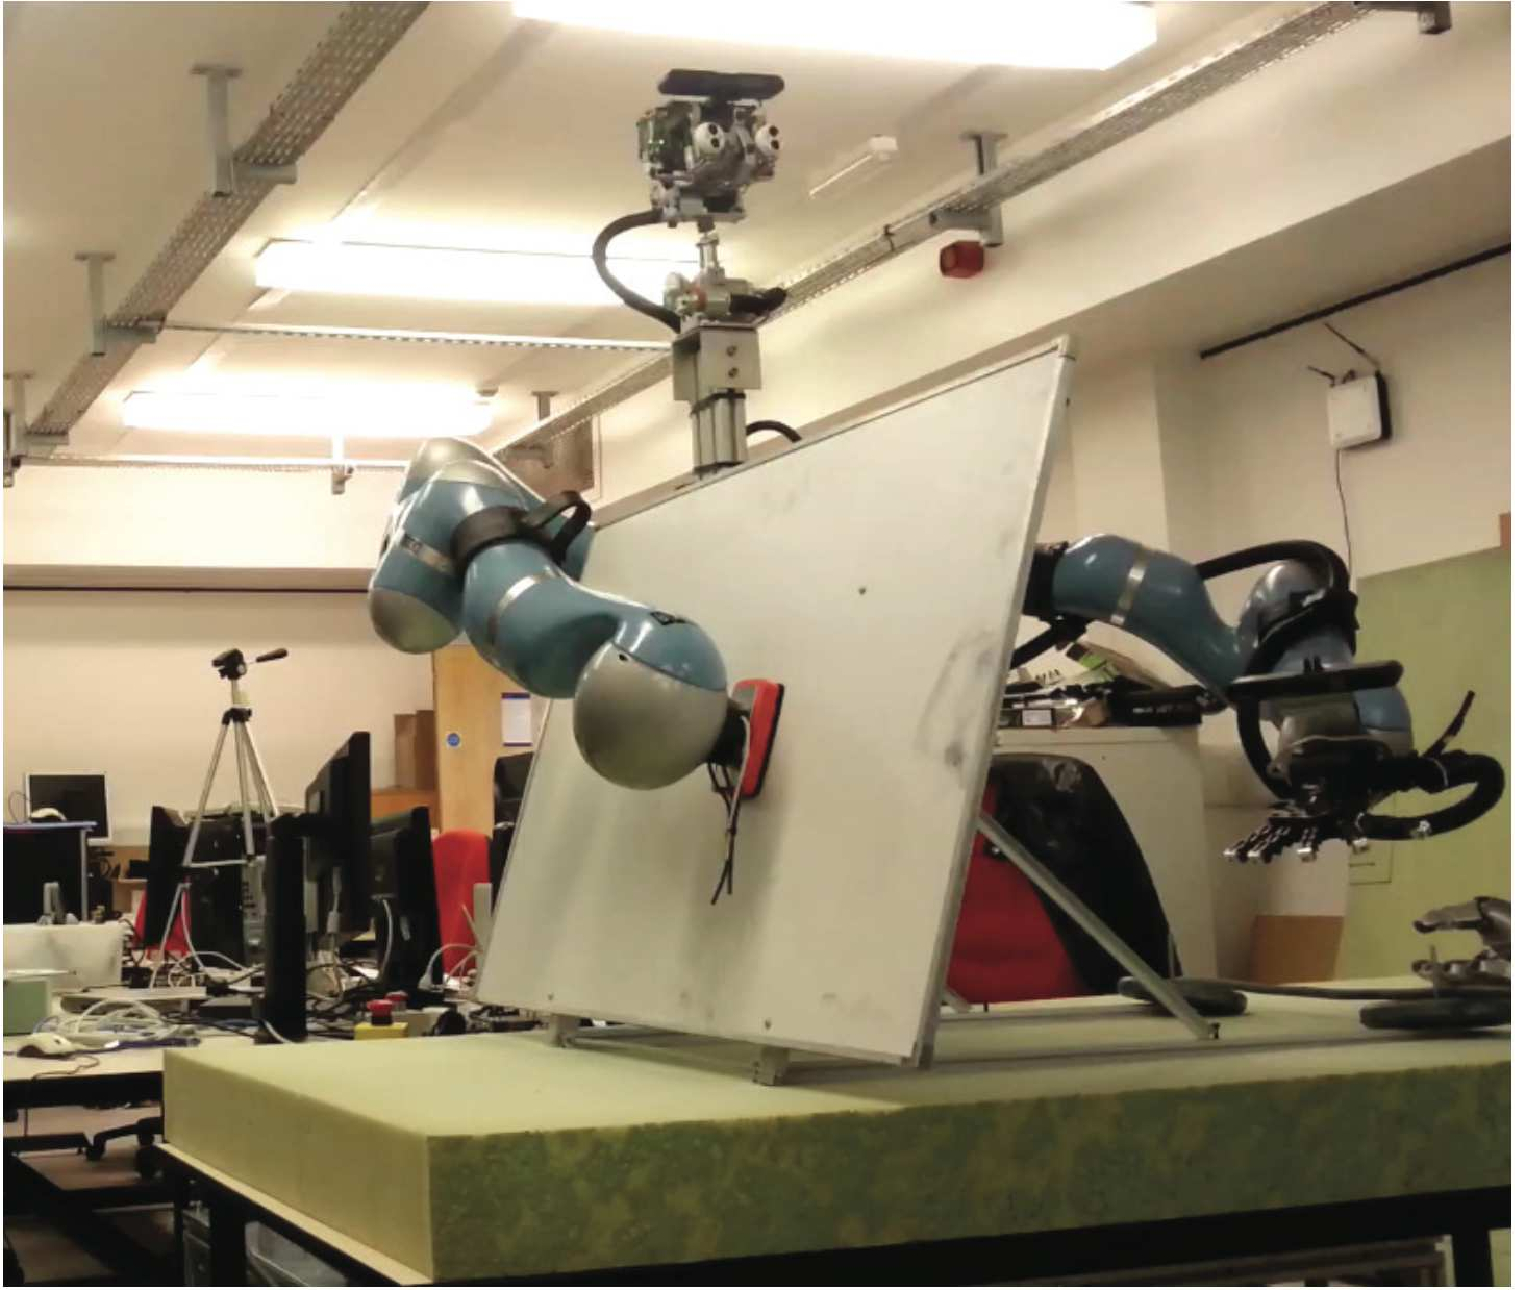
\includegraphics[width=0.65\textwidth]{images/whiteboard.pdf}
  \caption{Experimental setting. The right arm of the humanoid
    platform Boris is used, and placed the board in between its two arms so that the z
    axis of the robot end effector frame, the z axis of the robot base frame
    and the axis orthogonal to the board are parallel.}
  \label{whiteboard}
\end{figure*}









